% TODO: follow Beamer Users' Guide!

% Settings
\documentclass[11pt]{beamer}

% packages
\usepackage[utf8]{inputenc}
\usepackage{amsmath}
\usepackage{amsfonts}
\usepackage{array}
\usepackage{booktabs}
\usepackage{bxdpx-beamer}
\usepackage{colortbl}
\usepackage{dcolumn}
\usepackage{floatrow}
\usepackage{geometry}
\usepackage{graphicx}
\usepackage{hyperref}
\usepackage{multirow}
\usepackage{natbib}
\usepackage[normalem]{ulem}
\usepackage{pdflscape}
\usepackage{rotating}
\usepackage{setspace}
\usepackage{siunitx}
\usepackage{subfigure}
\usepackage{tabularx}
\usepackage{tcolorbox}
\usepackage{threeparttable}
\usepackage{ulem}
\usepackage{wrapfig}
\usepackage{xcolor}
\tcbuselibrary{fitting}


\PassOptionsToPackage{height=1.4cm}{beamerouterthemesidebar}  % custom header size
\usetheme{PaloAlto}  
\usecolortheme{default}
\usefonttheme{structurebold}
% \setbeamercovered{transparent}
\setbeamertemplate{caption}[numbered]
\setbeamertemplate{footline}[frame number]
\newcommand{\indicatewidth}[1]{\thickhrulefill{#1}\thickhrulefill}
\newcommand{\thickhrulefill}{\leavevmode\leaders\hrule depth-1.2pt height 3.2pt\hfill\kern0pt}
\newlength{\mytotalwidth}
\mytotalwidth=\dimexpr\linewidth-5mm
\newlength{\mycolumnwidth}
\mycolumnwidth=\dimexpr\mytotalwidth-5mm

\renewcommand<>{\sout}[1]{
  \temporal#2{\invisible{#1}}{#1}{\beameroriginal{\sout}{#1}}
}

%------------------------------------------------------------
% This block of code defines the information to appear in the
% Contents of the title page
\title[Nomination under Dual Listing]{
	Insurance Tickets: \\ Parties' Nomination Strategies in Japan's Mixed-Member Electoral System
}
\author[Dai Sasaki (UTokyo)]{ \href{https://dxxsxsxkx.github.io/}{Dai Sasaki}}
\institute[UTokyo]
{
    Graduate Schools for Law and Politics \\
    The University of Tokyo
}
\date[APSA 2024]{APSA Annual Meeting (Sep 6, 2024)}

\begin{document}

% Title
\frame{\titlepage}

\section{Overview}

% Overview
\begin{frame}{Today's Talk}  % TODO: fix

\begin{itemize}
	\item \textbf{RQ.} How do parties nominate candidates in the PR tier of Japan's mixed-member systems? 
	
	\item \textbf{Case.} House of Representatives election, 1996-2017
	
	\item \textbf{Findings.} 
	
	\begin{itemize}
		\item Parties are motivated to prioritize senior / incumbent candidates; 
	
		\item \alert{Dual listing} incentivizes parties to give \alert{insurance tickets} to these candidates. 
	
	\end{itemize}

	\item \textbf{Implications.}
	
	\begin{itemize}
		\item Legislative turnover; 
		
		\item Minority representation.
	\end{itemize}
	
\end{itemize}

\end{frame}


% Theory
\section{Theory}

\begin{frame}  %TODO: fix
	\frametitle{Japan's Mixed-member System}
	\begin{itemize}  
		\item The 1994 reform
		
		\item SMDs (SNTV) + PR blocks (closed lists)

		\item Mixed-member majoritarian (MMM)
				
		\item \alert{Dual listing}  
		
		\begin{itemize}  
			
			\item Can nominate candidates simultaneously in the two tiers
			
			\item Can give any of dual-listed candidates the same rank within a list 
			
			\item ``Best-loser" rule to decide winners among equally-ranked candidates
			
			\item Very common 
		\end{itemize}
	\end{itemize}
\end{frame}

\begin{frame}{Dual Listing is Very Common}
	\begin{figure}[H]
		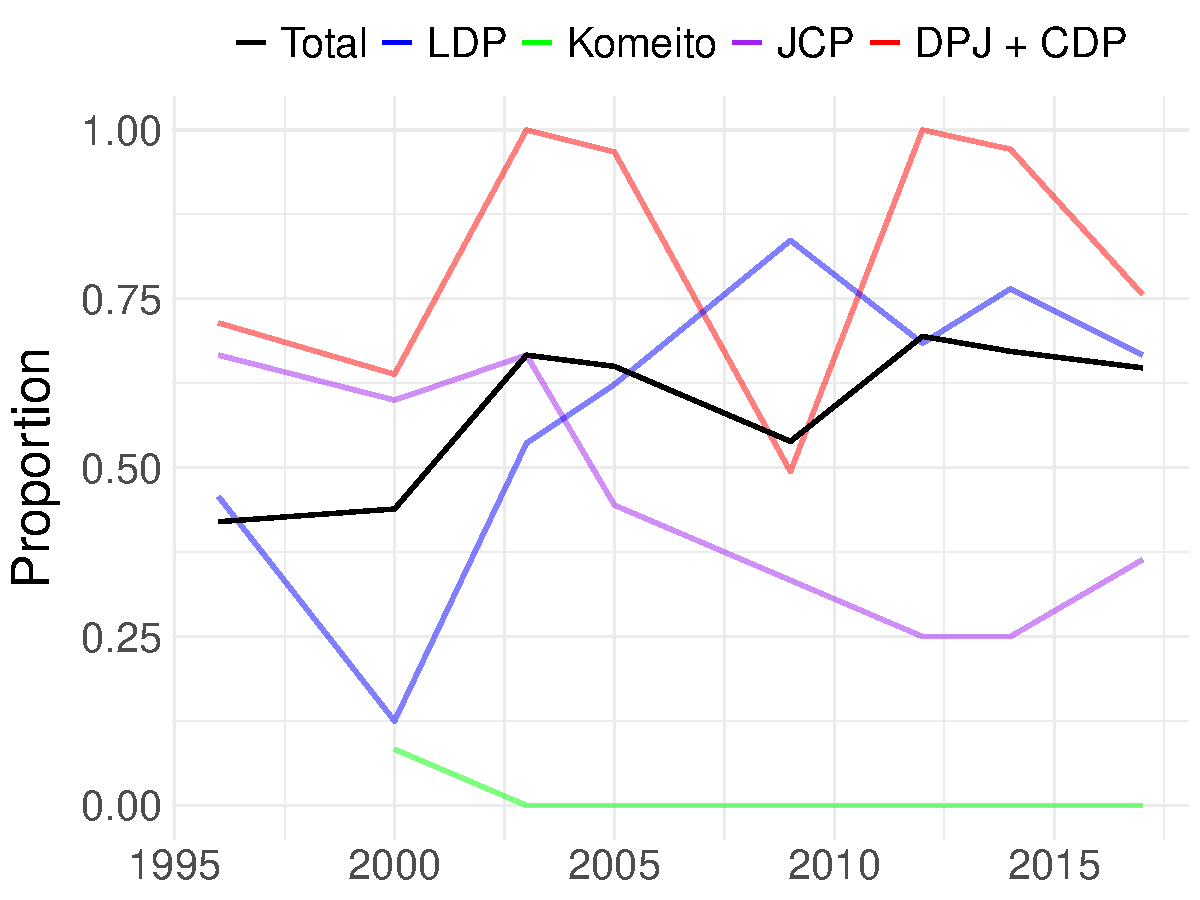
\includegraphics[width = 0.8\textwidth]{../figure/slide/dual_nomination.pdf}
		\caption{Proportion of Dual-Listed Winners}
	\end{figure}
\end{frame}

\begin{frame} 
	\label{Main claim}
	\frametitle{Theoretical Expectation}  
	\begin{alertblock}{Claim} 
		\begin{itemize}
			\item Parties are motivated to prioritize senior / incumbent candidates; 
			
			\item Dual listing incentivizes parties to give second chances to these candidates. 
		\end{itemize}
    	\end{alertblock}

	\begin{itemize}
		\item Parties care about post-election goals. 
		
		\begin{itemize}
			\item Policies, ministerial posts, legislative bargaining, ...
		\end{itemize}
		
		\item Senior politicians are generally better equipped with resources. 
	\end{itemize}

\end{frame}

\begin{frame}{Hypotheses}  
\begin{itemize}
	\item \textbf{Dual listing}
	\begin{enumerate}	
		\item[H1.] Senior candidates are more likely to be dual-listed.

		\item[H2.] Incumbents are more likely to be dual-listed. 
		
	\end{enumerate}

	\item \textbf{List rank}
	\begin{enumerate}		
		\item[H3.] Senior candidates are ranked higher. 	

		\item[H4.] Incumbents are ranked higher. 
				
		\item[H5.] Dual-listed candidates are ranked higher. 

	\end{enumerate}
	
	\item H1 - 5 should apply to all parties. 
	
	\item H1/3 should be less applicable when parties recently lost government / had internal disputes. 
	
\end{itemize}
\end{frame}

\section{Data and Method}

\begin{frame}
	\frametitle{Empirical Strategy}		
	\textbf{Data.} the Reed-Smith JHRED (Reed and Smith, 2018)
	\begin{itemize}
		\item PR candidates
				
		\item 1996, 2000, 2003, 2005, 2009, 2012, 2014, 2017
	\end{itemize}
	
	\textbf{H1 - 2.} Logistic models
	\begin{itemize}
		\item DV: candidate $i$'s dual-listing status 
			
		\item IV: candidate $i$'s N of past wins; incumbency status
						
	\end{itemize}
	\textbf{H3 - 5.} Negative binomial models
	\begin{itemize}
		\item DV: candidate $i$'s list rank 
					
		\item IV: candidate $i$'s dual-listing status; N of past wins; incumbency status
			
	\end{itemize}
	
	\textbf{Controls.} female dummy, district magnitude, year and party FEs

			
\end{frame}


\section{Result}

% TODO: H1 + H2 together here
\begin{frame}  
	\frametitle{Senior Candidates (H1) and Incumbents (H2) More Likely to be Dual-Listed}
	
	\begin{itemize}
		\item Male, LDP, Tokyo Block ($M = 20$), 2012
	\end{itemize}
	
	\begin{figure}[H]
	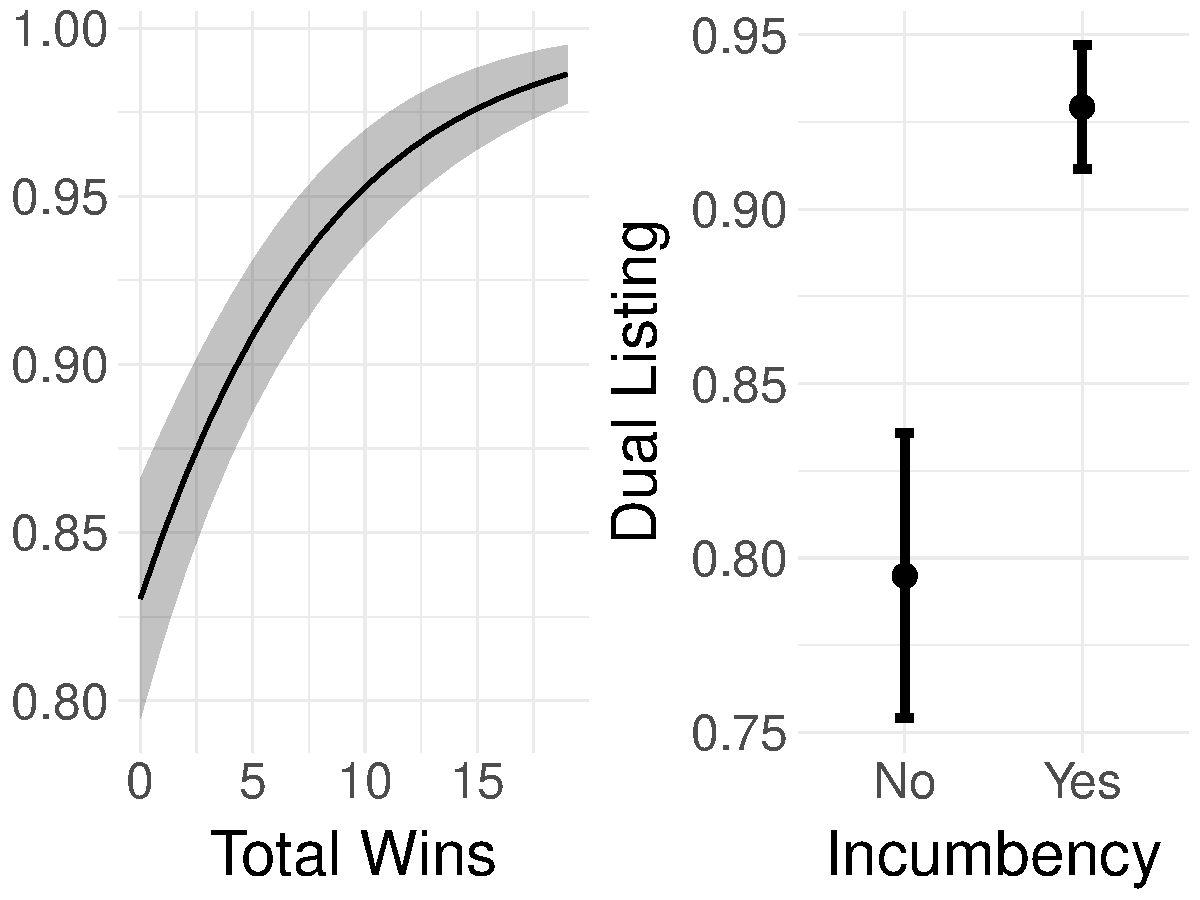
\includegraphics[width = 0.8 \textwidth]{../figure/slide/h1_h2.pdf}
    	\end{figure}
	
\end{frame}

% TODO: H3 - 5 together here

\begin{frame} 
	\frametitle{Senior Candidates (H3), Incumbents (H4), Dual-listed Candidates (H5) Ranked Higher}
	
	\begin{figure}[H]
	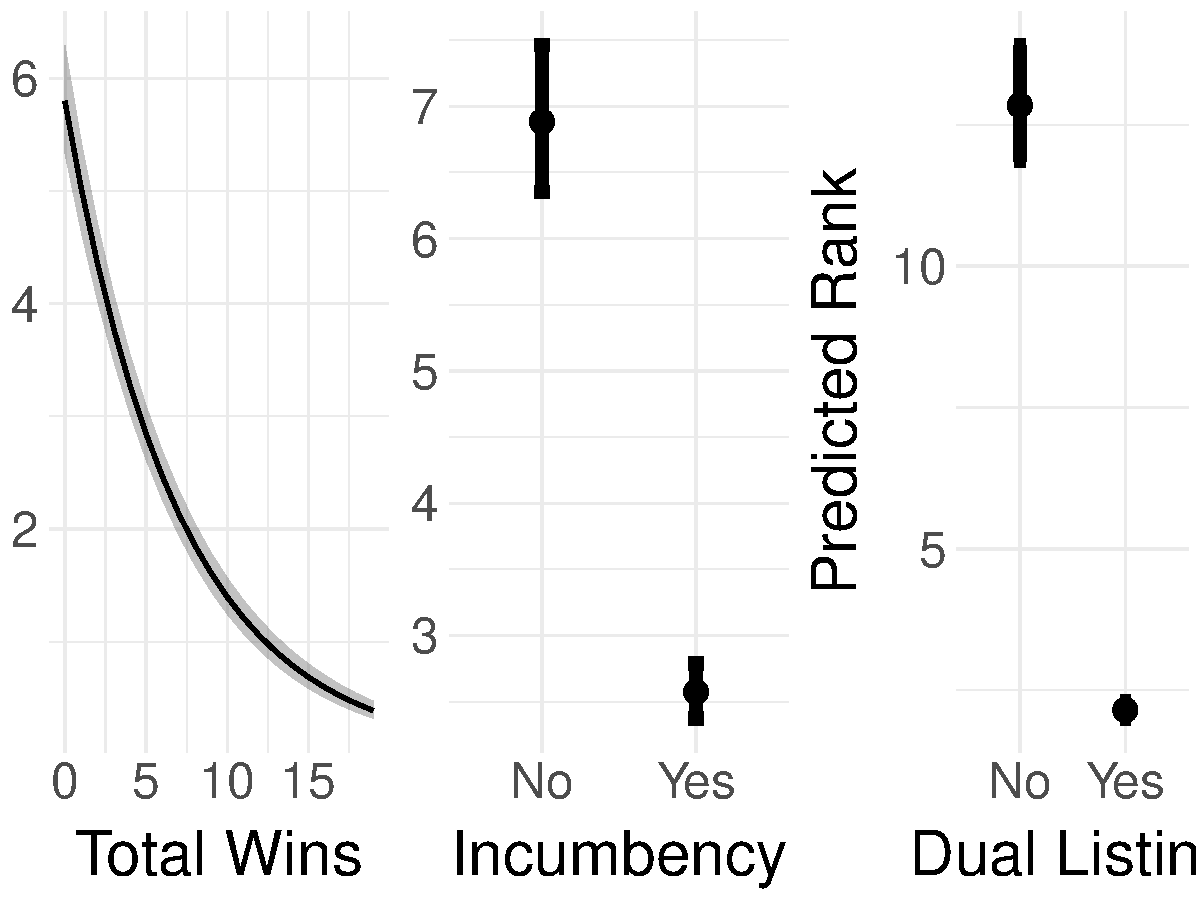
\includegraphics[width = 0.8 \textwidth]{../figure/slide/h3_h4_h5.pdf}
    	\end{figure}
	
	\begin{itemize}
		\item H3 / 4 hold after controling dual-listing status. 
	\end{itemize}


\end{frame}

% Party- / election-specific analyses
\begin{frame}  % TODO: add
	\frametitle{Election- and Party-Specific Analyses}
	
	\textbf{Findings:}
	\begin{itemize}
		\item Many parties prioritize senior and incumbent candidates, but only majority-seeking parties turn to dual-listing to do so: 
		\begin{itemize}
		\item LDP / DPJ - CDP: H1 - 5 applicable
		
		\item JCP (/Komeito): H3 - 4 applicable
		\end{itemize}
		
		\item Parties prioritize senior and incumbent candidates even when the door of opportunity is open: 
		\begin{itemize}
		\item H1 - 5 applicable to LDP in 2005 / 2012 elections
		\end{itemize}
		
	\end{itemize}

\end{frame}

\section{Discussion}

\begin{frame}{Discussion}

\begin{alertblock}{Findings} 
	\begin{itemize}
		\item Parties are strongly motivated to prioritize senior / incumbent candidates; 
			
		\item Dual listing incentivizes \textbf{majority-seeking parties} to give second chances to these candidates. 
	\end{itemize}
\end{alertblock}

\textbf{Implications: }

% implications here
\begin{enumerate}  
	\item Lower legislative turnover; 
	
	\begin{itemize}
		\item Limited N of candidates parties can nominate. 
		\item Priority on returning candidates = fewer new candidates. 
	\end{itemize}
			
	\item Lower minority representation. 
	
	\begin{itemize}
		\item Follows from lower turnover. 
		\item c.f., representational advantages of PR systems. 
		\item e.g., youth underrepresentation (more details in the paper!)
	\end{itemize}
						
\end{enumerate}

	
\end{frame}


\appendix

\end{document}